% READ ME, PLEASE !!!!
% This document is based on the LaTeX format of Mark T. McLaughlin's thesis
% which was made with WinEdt 5.4, October 2005.  This top section is his
% comments.
%
% 1) IF YOU CAN'T FORMAT SOME PART OF YOUR THESIS ACCORDING TO THE CSULB
%    THESIS GUIDELINES:   DON'T WORRY!!
%    Just rewrite the crap in MSWord. The command, \usepackage{times}
%    puts everything in the same font as the times roman used by MSWord
%
% 2) There are a few SMALL PROBLEMS with the
%    table of contents, list of figures, and list of tables. The problems are
%    a) appendix subhead titles are not supposed to be included in the table of
%    contents, b) figures in the appendices are not supposed to be included
%    in the list of figures, and c) tables in the appendices are not supposed to be
%    included in the list of tables. -EASY SOLUTION: Make up a phony appendix, say
%    phonyAppendixA, which is blank, but the same number of pages as your real
%    appendix A. (Similarly, do the same with appendix B, appendix C, etc...)
%    Then at the end of this file, main.tex, comment out your real
%    appendix A, and uncomment this phony appendix when you LaTex your document
%    for the purposes of generating a table of contents, list of figures, and
%    list of tables. Then when you want to LaTex the rest of your real document,
%    comment out your phony appendices, and uncomment your real appendices.
%
% Everything else passed the thesis office inspection!!! -Bibliography, Signature page,
% Equation numbering, figures, tables, margins, all that junk......
% Thanks Yamato Matsuoka for creating such a nice thesis template!
%
% MORE HELPFUL STUFF:
% TIPS FOR MAKING FIGURES AND TABLES
%   AUTOCAD:
%       In Windows: autocad -> HP color laserjet postscript -> print to filename.ps
%       In Linux: pstoedit -f xfig filename.ps filename.fig
%                 xfig filename.fig
%        in xfig: export -> filename.eps
%        put filename.eps in LaTex document
%
%   EXCEL: excel -> print to postscript (in printer settings click on eps postscript)
%       In Linux: pstoedit -f xfig filename.ps filename.fig
%        in xfig: export -> filename.eps
%        put filename.eps in LaTex document
%

%% =====================================================================
%% Thesis --- Main LaTeX File  ver 0.1
%%                 Date: 9/1/2012 started
%% =====================================================================

\documentclass[12pt]{csulb_thesis}
%\documentclass[12pt]{report}  %% regularly use this
\usepackage{amsmath}   %% mainly to use align environment
\usepackage{amssymb}   %% to use \boldsymbol
\usepackage{times}
%\usepackage{txfonts}
%%% txfonts converts default CM fonts to the followings
%%  Computer Modern Roman      -->  Times
%%  Computer Modern San Serif  -->  Helvetica
%%  Computer Modern Typewriter -->  Corresponding Typewriter Font


%\usepackage[dvipdfm]{color}  %% if you like

%\usepackage[dvips]{graphicx}
% \usepackage[dvipdfm]{graphicx}
\usepackage{graphicx}
\usepackage{hyperref}

%% For printing use   [Option `hyperref.sty' is needed]
\hypersetup{colorlinks=false}

% -------------
% For pdfLaTeX
%\usepackage[pdftex]{graphicx,color}
%\usepackage[pdftex,colorlinks]{hyperref}
% -------------

%%
%\allowdisplaybreaks[1]
%%% \allowdisplaybreaks[n] ... allow pagebreak within eqnarray/align environment n = 1~4

\nonstopmode  % Keep compiling even when errors occur


%% ----------------------------------
%%            Newcommands          %%
% \newcommand{\vect}[1]{\boldsymbol{#1}}  % vector (bold symbol)
% \newcommand{\uvec}[1]{\hat{\vect{#1}}}  % unit vector (bold & hat)
% \newcommand{\mytxt}[1]{\texttt{#1}}
% \newcommand{\mybold}[1]{\textbf{#1}}
% \newcommand{\prof}[1]{Dr$.$ {#1}}
% \newcommand{\myA}[1]{A$({#1})$} %A(t), the acoustic signal from the microphone
% \newcommand{\myB}[1]{B$({#1})$} %B(t), a signal N times the freq of A(t)
\newcommand{\tab}{\hspace*{1.5em}}

%% ----------------------------------


%% ----------------------------------
%%          Author's Info          %%
\title{Efficiently Managing the CECS Computer Labs}
\author{Nathan Pickrell}
\gradmonth{December }  % month & year of the graduation
\gradyear{2012}  % month & year of the graduation
\department{Department of Computer Engineering and Computer Science} % department
\degree{Master of Science} % CSULB degree
\bachelor{B.S.}  % bachelor degree (abbreviated)
\bacheloryear{2010}  % The year bachelor degree was given
\undergraduniv{California State University, Long Beach} % university where the degree was earned
%% ----------------------------------



%% ---------------------------------%%
%%       Thesis Committee           %%
\firstmember{Dennis Volper, Ph.D. (Chair)} %%% Don't forget to put (Chair) at last
\deptfirst{Computer Science}

\secondmember{Kenneth James, Ph.D.} 
\deptsecond{Computer Science}

\thirdmember{Tracy Maples, Ph.D.} 
\deptthird{Computer Science}

\deanname{Kenneth James, Ph.D.} 
\deandept{Department Chair, Computer Science}
%% ----------------------------------


%%------------- Begin Document -------------------%%
%%                                                %%
\begin{document}
\abstract{\thispagestyle{empty}

The CECS computer labs require efficient management to run effectively. The technicians maintaining these labs have a lot of issues they must deal with from difficulties dealing with Faculty to frequent software updates. This paper describes the author's work as a technician and how he improved the labs. 
}
\maketitle

%\pagenumbering{arabic} %%%%%%% Comment Out if the abstract is one page long %%%%%%%%%%
%\pagestyle{empty}     %%%%%%% Uncomment   if the abstract is one page long %%%%%%%%%%


%%%---- Insert them if \signaturepage is not used ----
%\pagenumbering{roman}
%\setcounter{page}{2}   %%% Adjustment of Page numbering
%%%----

\signaturepage
% \include{acknowledgement}
\tableofcontents 
%\listoffigures
%\listoftables

%%%%%%%%%%%%%%%%%%%%%%%%%%%%%%%%%%%%%%%%%%%%%%%%%%%%
%%    This is manually inserted TOC entry!        %%
\addtocontents{toc}{\protect\contentsline{chapterhead}{\chaptername}{}{}}
%% the last {} may be removed if `hyperref.sty' is NOT used.
%%%%%%%%%%%%%%%%%%%%%%%%%%%%%%%%%%%%%%%%%%%%%%%%%%%%

%%%% Similarly, the following should be inserted somewhere in the document
%%%%%%%%%%%%%% TOC entry ! %%%%%%%%%%%%%%%%%%%%%
%%\addtocontents{toc}{\protect\contentsline{chapterhead}{\chaptername}{Page}{}}
%%%%%%%%%%%%%%%%%%%%%%%%%%%%%%%%%%%%%%%%%%%%%%%%

%%%% Or, insert the following if page breaking occurs in appendix entries
%%%%%%%%%%%%%% TOC entry ! %%%%%%%%%%%%%%%%%%%%%
%%\addtocontents{toc}{\protect\contentsline{chapterhead}{\null}{Page}{}}
%%%%%%%%%%%%%%%%%%%%%%%%%%%%%%%%%%%%%%%%%%%%%%%%


\clearpage \pagenumbering{arabic}
%\chapter{Introduction} \label{ch:introduction}



Title: Introduction: The Problem

-Student oriented labs.
The CECS labs are student oriented.  Some research can be done with them, but we focus primarily on coursework.  We restrict privileges on them but have a fairly liberal security policy so that students can do development work. 

\subsection{Limited faculty Testing}
One of the main problems we have with faculty is a lack of feedback during the architect phase for lab images.  Requests for changes during the time we build the labs come from only a small handful of faculty.  Most faculty will wait until a week before the semester starts before making change or update requests.  Some of them will even wait until the semester starts (although these are often ignored from faculty that are repeat offenders).  

We understand why this occurs.  Most faculty are not paid during the summer months and are therefore under no obligation to work.  However, this does not excuse them from submitting requests at the end of the previous semester.  They are also never given any sort of penalty for doing this especially if they are tenured.  Part time faculty also have the problem where they are not told what classes they will be teaching until a few days before semester starts or even after it starts.  

In any case, this is a problem for us because we have very limited amount of testing on our lab images.  We often do not have the knowledge base to test software needed for classes because we do not understand it.  We research as much as we can and hope that that is enough.  We also have a relatively fast lab cloning procedure to recreate the labs in the event of emergency when the semester starts.  However, in many cases we must ignore requests from faculty members until the next iteration of the lab images the following semester.

\subsection{Staff and Faculty Turnover}
In addition we also have the problem of short faculty turn over.  Our part timer lecturers do not stay if their reviews are poor.  This is good for the students and usually if they are not well liked by the students, they are not well liked by the staff either.  The problem with this turn around is that we do not have a complete list of faculty.  The list is changed often and no attempt is made to keep it updated.  This means that we cannot reliably send out email to all faculty to explain issues or give instructions.  

\subsection{Mixed Environment}
We have the fourth floor of the Engineering and Computer Science building dedicated to our labs.  We have 3 Linux labs of 30 workstations each, 4 Microsoft Windows labs of 30 workstations each, and an Apple iMac lab of 25 workstations.  Operating systems on these workstations are very different from one another.  This requires experience in many areas and is virtually impossible for a single staff member to accomplish alone.   

\subsection{Frequent Software Updates}
There are numerous pieces of software to install and maintain on our workstations.  We do this by creating master lab images for each platform and deploying them through a cloning procedure.  Maintenance of these master images is time consuming as there are frequent software updates to software on them as well as to the operating systems.  

\subsection{Limited Staff}
We have a limited amount of staff available to us.  This is not uncommon in industry.  IT departments are often kept lean because they are seen as an expense.  This results in limits to how much work can be done and how many technicians are available to support a number of workstations.  We improve this situation through automation, but there is only so much we can automate.  Often, we have to postpone needed updates and feature requests until we have time.   




Despite the problems we have, the situation is not hopeless.  We do as much as we can to keep things running efficiently.  This paper will document the various steps we take to do so.  However, it will focus on the Linux environment and only touch briefly on other platform.  

\chapter{The Documentation Solution} \label{ch:documentation_solution}
\section{Lab Documentation}\label{sec:documentation_solution}
\subsection{Overview}
With any lab management, documentation and procedures need to exist.  For example, if master lab images exist, full sets of instructions need to exist to describe how to rebuild the master from scratch at any point during the process.  That said, a secure place needs to exist to hold this documentation.  At a minimum, it needs to be in a directory somewhere that is periodically backed up.  More advanced documentation solutions may use online wikis or even code repositories for revisions along the way.  In the CECS lab environment, we have a good backup system in place for user accounts, so we created a user "conf" to store documentation in.  

\subsection{Special Documentation User}
The conf user can be created in the same way as a standard user account.  The disk quota is unlimited, however, that is not a problem because the account only stores text documentation.  In our case, conf is used to hold a student’s skeleton directory, therefore, a quota is not applied.  Since conf is a network user account, it is available from all machines that have Network Information Service (NIS) and Network File System (NFS) mounts set up.  

Accessing the account can be done in several ways.  If an administrator can become root on a machine where conf is accessible from, they can ”su - conf” on the machine to become conf.  The rlogin command can be used assuming a user is in conf’s .rhosts file.  The modern equivalent of rlogin, Secure Shell (ssh), can be set up by adding an authorized administrator’s public key to conf’s ”authorized keys” file.  

In conf's home directory, we created a folder called "admin" to hold administrative documentation.  Subfolders for the various lab builds exist.  We have folders for Linux labs, Mac labs, a few notes on the network, patches, the print servers, and the web servers.  Other directories are created as needed.  These directories should contain such things as system build notes, system patching notes,\footnote{Notes will include both distribution patches and manual fixes} supporting documentation,\footnote{These include things like user manuals and web links} or just general system notes.  Storage of the actual system patches can become quite large for a network filesystem.  It is usually much more efficient to have a dedicated file server to store large patches and distribution images.  In our implementation, all of these folders are set to world readable.  We do not store any sort of password or key information and do not have a problem with students being able to read how our labs are set up and managed.  Security through obscurity is not really security at all.  

\subsection{Alternatives}

Alternatively, the information can be stored on a wiki.  Setting up a wiki requires a webserver and usually needs php and mysql support.  The setup of the wiki can become somewhat convoluted depending on the configuration.  The advantage of the wiki is that it can be accessed by any web browser.  It may even be stored on the same server used for the support website.  It is probably not a good idea to open this webserver to the Internet since it has many more security vulnerabilities than flat files.  In addition, because so many components are involved, backing up the wiki can become very cumbersome.  To date, we have not been able to correctly back one up in CECS labs without backing up the entire webserver.  

Another alternative is to just use a code repository such as Subversion or Git.  These services require complex configurations to set up properly.  However, the advantage of using these services is the revisioning and editing ease.  These services can even be integrated into a web server to get the advantages of both.  For our purposes though, we found that simple text files work adequately so long as they are periodically backed up.  

\section{Student and Faculty Help}\label{sec:student_faculty_help}
\subsection{Introduction}
Regardless how well structured a lab is, user support is necessary for problems and potential confusion.  This support may come in the form of a tech support email, ticketing system, website with an FAQ, or some fix utilities.  CECS labs offer a website, a tech support email, some text files with instructions, and some Linux fix scripts.
\subsection{Support Website}
The first line of support is a website.  The site should have at a minimum a frequently asked questions (FAQ) section.  FAQ pages should be very easy to find and be clearly visible.  This is the equivalent of a README file with a software distribution.  This FAQ section should answer such things as getting started, creating an account, troubleshooting accounts, resetting passwords, or answering various issues users may commonly have.  It should also have bold and/or red lettering to highlight important procedures and rules students should follow, e.g. no food or drink in the labs. 

The website is unfortunately rather pointless if users do not know where it is (or that it even exists).  In academic environments, this can somewhat be remedied by having faculty members explain to students where to go in case of a problem, or provide a handout on basic lab usage.  Of course, many students will just ignore this.  A better solution\footnote{This solution works well in non-academic environments as well because it is easier in IT department to have systems labeled with hostnames.} is to just put a label on the front of every machine with the hostname, support website, and tech email.\footnote{Tech email can be replaced with ticket helpdesk url in environments that use one.}  This will hopefully lead users to the proper place rather than coming to the technicians.  It is very important that the support website be featured prominently with clearly legible text. 

In the CECS labs, we have a support site that is the default homepage for every user.  It has everything mentioned above, however, our problem is that it does not have the latest up to the minute updates.  We do the best we can but constant changes in our environment for each release make a completely accurate website unfeasible. We strive to be accurate within a few days of the changes.

\subsection{Support Email and Alternative}

Regardless how well put together a website is, it does not account for everything.  There has to be some method of contacting tech support to report problems and ask for troubleshooting help.  The simplest way to do this is by setting up a contact email.  However, in environments with more than one technician, this contact email has to have a forwarding list.  This way, email sent will go to all techs involved.  Emails lack the ability to inform all recipients if an email has been read, or in this case, if the problem addressed in the email has been resolved.  This may cause technicians to duplicate work.  This is not much of an issue with small tech shops, especially with each tech sticking to a specialty.  But in large organizations where IT support can exceed more than a few people, support emails can be inefficient.  A solution is to set up an email with a Reply-to field so that users always answer to the single tech email that forwards to all techs.  Not all email clients properly implement this feature and some of the most common clients ignore it entirely.

Thus, a ticketing system can be a better solution.  Tickets are opened through a custom interface, e.g. a support web application.  Users login to a ticket helpdesk and open tickets describing their problem.  They may select one or more categories of problems that their issue falls under.  From there, an IT support staff can login to the helpdesk as administrators and look for tickets to work on.  A good ticketing system also has in place mechanisms for leaving notes and attachments\footnote{Attachment capability is especially necessary for screen shots.} on how the problem was resolved and what the problem was.  More advanced features might include an interface for managers to login to the helpdesk and approve requests that require management approval.\footnote{Examples of actions needing management approval include production system updates, access management changes, and operating system configuration changes.}  Lastly, the ticketing system is easier to audit compared to long email trails and is practically a necessity in environments where strict compliance is needed.   

Ticket helpdesk systems usually do not work in small environments, especially academic settings because the system is often too confusing for students to bother with.  They will usually just ignore it and continue on despite a potential problem.  Faculty will most likely never use the system and will bypass the system by emailing the first technical support contact they can.  Thus, a ticket helpdesk is probably not feasible in our environment unless required as a campus wide regulation.  

\subsection{Fix Utilities}

Sometimes a lab load cannot handle certain configurations the students and faculty may impose locally.  Various configuration files may exist in their home directories and may override system defaults.  If the configurations are not set up correctly, various issues may occur.  Sometimes these configurations may not even be intentional.  Home directories may be migrated from one distribution to another and configurations may not be compatible.  Thus, a set of fix scripts is necessary to reset configurations to a default structure.  These scripts may be located on all lab machines, but updating them would require Secure Shell (SSH) pushes to keep machines consistent even with some other repository software.  If network mounted home directories are used, it is wise to create one or more utility users (for example, ``conf") whose files are left world readable and executable.  For example, students may have a faulty ``.gnome2" configuration that could cause the gnome window manager to malfunction.  A script called ``resetX" exists in conf's home directory ``~conf/" and is world executable.  Students can run ~conf/resetX from a machine that has conf's home directory mounted or automounted.  This script will delete a student's copy of the gnome configuration and pull in a working configuration.  The script could also have logic to determine if a student has a common problem in their configuration and correct the problem without overwriting the entire configuration.  A copy of this script can be found in Appendix~\ref{ap:lab_maintenance}. 

There are a variety of other useful scripts that could be put in conf's home.  For example, you could create a script that would restore all configuration files from a tested skeleton account.  Sometimes, NFS files become locked and students do not know how to unlock them.  A script to find and unlock the files would be very helpful.  Backup and restore scripts could be useful, especially if a nightly backup system is run.  Care should be taken as to where these scripts should reside, however.  If the script often changes it should be put in ~conf/ and shared over the network.  If the script is somewhat more permanent, it is often easier to just house the script locally.  The recommended location for these scripts is in ``/usr/local/bin/" where they are made world executable.  Thus, with each master image revision they will be updated if needed.  


\section{Print Servers} \label{sec:Print Servers}
\subsection{Overview}
At the core of every lab should be some sort of utility server.  This server should handle a variety of functions to serve the client machines in the lab.  In CECS labs, the most obvious function for these servers was printing, so we decided to call them print servers and name them psvr<lab room number>.  Printing is described in the lab printing section.  The rest of the Print Server functionality consists of:  DHCP, TFTP, PXE boot, NFS, Samba, Norton Ghost (for windows), and to function as NIS slaves.
\subsection{DHCPD Server}
The DHCPD server functions to hand out IP addresses to the client machines in the lab.  The DHCPD has to be on the same subnet as the clients due to how DHCP addresses work.  Clients send a broadcast on the local subnet to request an IP, and DHCPD responds.  It is possible for this broadcast to escape the subnet, but that requires the router (or layer 3 switch) to use an IP helper protocol.  This protocol maps broadcast requests to their origin subnets so that answers can be returned.  In CECS labs, we prefer to keep DHCPD on the same subnet in the event that if connection outside the lab is lost, clients can still function locally.  
\paragraph
In addition, the DHCPD server must hand out addresses based on Mac addresses.  This is because IP addresses are mapped to hostnames in DNS.  Hostnames should match the labels listed on the client machines.  This way, if a problem with a client machine is reported, Tech Support knows both where the machine is physically and how to reach it over a network.  IP addresses should not be handed out randomly for normal operations (though it could be done for cloning if static addresses are assigned later).  
\paragraph
Alternatively, static addresses can be assigned on a per machine basis during the cloning process.  The advantage to this is the clients will be on the network regardless what happens to the DCHPD server.  The disadvantage to this is the cloning process will require someone to manually enter an IP for each client at some point, and this will break the ability to do fully automatic lab installs.   Regardless how IP addresses are handled during normal operations, dhcpd must be turned on during cloning to support TFTP and PXE for network booting.  
\subsection{Network Booting}
One of the most important uses of the print server is cloning the labs.  Full details for that are listed in the cloning section, but the print server side is described here.  The core part of the cloning requires the ability for clients to network boot (netboot) from the print server.  
\paragraph
Netbooting requires 3 things:  DHCP (listed above), TFTP, and PXE.You will also need NFS for the cloning process.  DHCP is required because the machines do not know who is who and require an IP address to get started.  After they have successfully netbooted, the IP address they have can be changed to the one they actually need or be mapped automatically with dhclient if the print server knows their MAC address.  
\pargraph
TFTP (Trivial File Transfer Protocol) is required for loading the initial boot image.  TFTP has very little security and must be highly restricted on the print server.  It has no authentication and only allows downloading of specific files.  This is necessary because during netboot, clients do not have any sort of identification or credentials that they can use.  TFTP is only used for the loading of the boot image initrd (a ram disk) and associated configuration files used by PXE.  The lab image to clone with is transferred with NFS after the machine has fully booted.  
\paragraph
DHCP and TFTP are used to support PXE (Pre-boot Execution Environment).  This is the protocol used to support netbooting without the help of any storage device on the client.  Clients will go out and grab an IP from DCHP, then download a file listed in the Print Server's dhcpd.conf file.  That file (usually called pxelinux.0 or something similar) is then downloaded and executed.  It gets its configuration files, loads the ram disk containing the network boot filesystem, and loads the kernel.  From there, it is then usable as a stripped down Linux OS run fully from memory.  It can then be used to both create the master lab image and deploy the clones.  It can also be used to troubleshoot where a full installation is not available (though tools are limited to the size of the ram disk).
\subsection{Network File System}
The Print Servers also mount NFS shares from the core fileservers.  It uses automount for this because automount will periodically check if the mount fails and attempt a remount.  Linux clients can mount the Print Server shares, thus making them a relay.  However, we have found it easier to just authorize all lab subnets to mount the core server shares directly instead of using a Print Server as a middleman.  

\subsection{Samba Support}
Since the file servers are all Linux based with clients mounting via NFS, some compatibility is needed for Windows Clients to mount those shares.  Windows uses its own network file system called SMB (Samba).  This is not compatible with Unix NFS natively.  Thus, a translation of sorts is needed.  The Print Server handles this by mounting the NFS shares from the core servers and running a samba server that acts as a middleman for the Windows servers to mount.  The Samba server requires a fair amount of CPU and memory resources to do on-the-fly translation of NFS to Samba. As a result, we have equipped the Print Servers in the Windows labs to have quad core processors that can handle a large classroom full of Windows SMB file requests. These would not be necessary if Windows could natively mount NFS. Supposedly, they can in certain versions of Windows 7, but we have been unable to make it work.

\subsection{Norton Ghost:  Windows Alternative}
For installing Microsoft Windows, a Linux network boot image is insufficient.  Instead, a tool called Norton Ghost is booted by all the clients and used to do a byte by byte copy of the Windows image to all the Windows clones.  This tool is proprietary and its workings are held secret by the Symmantec corporation (it is free to use though).  However, it is useful for Windows administrators who may not necessarily know Linux that well.  One advantage it has is the use of multicast to send the image to all clients at once instead of one at a time.  The disadvantage to this is that if a client misses a packet, it must be cloned again.  An alternative to using Norton Ghost is just netbooting to Linux and using dd to do a binary copy of the Windows image.  This would be problematic on hard drives of different sizes as the image could only be the size of the smallest hard drive used in order to remain compatible.  

\subsection{NIS Slave}
Print servers are important for authentication because they provide NIS information to the rest of the lab.  The core server holding the NIS namemaster does not grant login information to all machines.  Instead, it designates each Print Server in a lab as an NIS slave.  This way, the Print Servers themselves can authorize the clients under them.  This hierarchy grants obvious advantages to administrators, especially if the administrators themselves have a hierarchy.  

\section{Filesystem Management} \label{sec:filesystem_management}
\subsection{Background}
Often in a lab environment, particularly an educational one, users will benefit from having persistent storage so that they may work day to day.   File storage has become less important in recent years because storage is now commercially cheap.  Nowadays, flashdrives that can hold gigabytes of data can be bought for less than one dollar per GB.  In addition, with the advent of cloud storage services, many companies offer free storage online.  Additionally, code repositories not only facilitate filesystem management, but can help with revision archiving.  However, it is still very convenient to have a small amount of storage between computers in a set of labs.  

For network storage, central file servers are the most common.  Some implementations use distributed storage across an entire lab's hard drives.  This method requires a number of security and redundancy considerations and should only be considered if the support staff is able to maintain it.  The central file servers in our environment run Suse Linux and export user home directories with NFS.  

\subsection{NFS Exports}
In the CECS labs, there are 3 file servers each holding 7 hard drives apiece.  Each drive contains home directories for students and faculty members to use daily.  The drives do not have any special configuration and are simply formatted with a standard Linux filesystem.  Each drive is exported via NFS and its exports are only available within CECS lab subnets.  Because of this, we can set the exports to run in insecure mode for compatibility reasons.  We also export with "root\_squash" enabled for all but one subnet.  This prevents an attacker who may have gained root privileges from damaging or stealing all of the files held.  All of this is configured in the "/etc/exports" configuration file on each fileserver.  The simplicity of the configuration has made this system run well for roughly a decade.  Most issues arise from hard drive failures and client configurations.

\subsection{Home Directory Changes}
Although "root\_squash" is useful for preventing possible disasters, "no\_root\_squash" is highly useful for fixing things affecting all students.  For example, when updating between the Linux distributions Fedora to Ubuntu, students still kept the same home directory with the same set of configuration files.  Files that functioned in Fedora broke various features of Ubuntu (most often with window managers).  These file issues are consistently the same with most students. Students can be given instructions, perhaps on the support FAQ, on how to fix issues on their own, but that inevitably leads to many emails to tech support.  Instead, it is useful to have a server or small subnet that has permission to mount student home directories on file servers with "no\_root\_squash."  That way, root can then make edits on all student homes at once via a script.  This script needs to have a lot of checks in place to ensure that it fixes the problem without interfering with other processes.  It also needs highly verbose logging to figure out if anything went wrong.  In its simplest form, this script would just loop through a list of affected student home directories, change directory (cd) to each of them, and run the necessary commands to fix the issue.  A copy of a simple script can be found in Appendix~\ref{ap:lab_maintenance}.

\subsection{Disk Quotas}
Total space for network storage is highly limited in the CECS labs.  Although hard drives have come down in price considerably, with almost 1500 accounts at any given time, a disk quota is necessary.  We set a conservative disk quota of 512 megabytes (MB) for each student and 1 GB for each faculty member.  This may seem small considering the price per GB, but students write code in text files.  They are not doing heavy picture or video editing, so that amount of space has been sufficient so far.  However, we recently noticed that web pages are are becoming larger and browsers are caching more as a result.  Mozilla Firefox in particular now sets its cache limit at 1 GB.  Thus, students are filling up their quotas quickly just by visiting websites.  We have modified the cache in browsers to an older 50 MB limit, but we realize our file servers will need to be upgraded in the next couple of years to keep up with increasingly larger files.  Typically, when the fileservers collectively become more than half full, we begin to worry about space.  

\subsection{Automount}
We use the automount tool on our workstations and servers to mount file shares from our core fileservers.  The automounter has several advantages over the classic method of relying on the file system table (fstab).  The fstab mounts immediately from when the /etc/fstab is read on system startup.  This uses system resources when a mount is not being utilized.  In addition, if a mount fails, it will not remount until either a system administrator (sysadmin) remounts it manually or the system restarts.  The automounter addresses both these issues.  It runs as a daemon in the background and waits for NFS requests by other processes.  It handles the given request and only mounts the file share that it needs to.  In addition, if the mount fails for some reason, it actively attempts to mount again in case there was a random network issue.  The /etc/auto.master configuration file governs the automounter's behavior.

\subsection{Backups}
We have two stages of backups.  One backup is done nightly to a set of file server clones.  These clones have the same hard drive and export configurations as the main file servers.  Though it has never been necessary, theoretically, if a file server goes down, we need only change the hostname of the backup to get it up and running again.  The other backup is done every Saturday to a set of hard drive arrays attached via a Small Computer System Interface (SCSI) cable.  Figure~\ref{fig:FileserverLayout} shows our fileservers and backup fileservers.

\begin{figure}
  \begin{center}
    \scalebox{0.7}{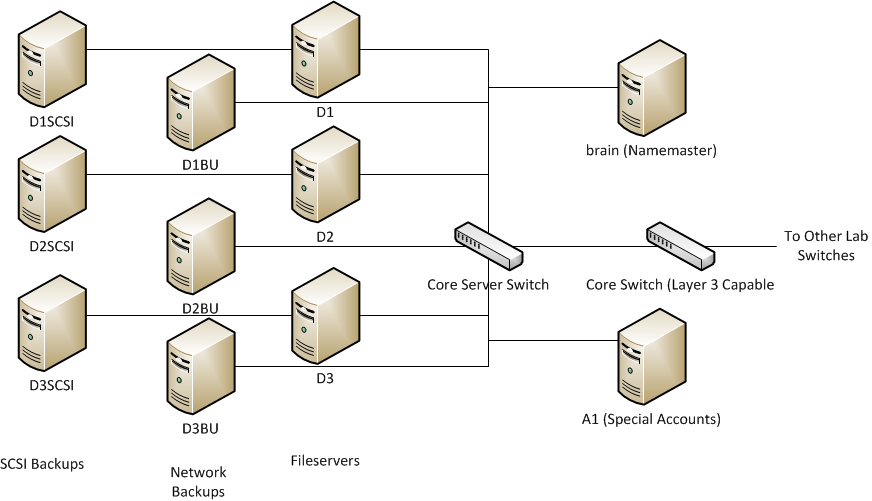
\includegraphics{../figures/FileserverLayout.png}} 
  \end{center}
  \caption{Core fileserver layout.}
  \label{fig:FileserverLayout}
\end{figure}

Both backups are done with the tar command to keep things simple.  Because this system is so uncomplicated, it is simple to maintain and troubleshoot.  Students are able restore files from backup by running the "retrieve" command and restore their entire home directory with the "shotgun" script.\footnote{A copy of the shotgun script can be found in Appendix~\ref{ap:lab_maintenance}.}

Though they do require periodic checks by our technicians, their simplicity makes our file servers the most stable point of our environment.  Unfortunately, due to higher space demands, their current capacity is quickly becoming insufficient.  Likely, once decommissioned, we will have no more file storage unless funding is appropriated for more space.  Without file storage, students will have to procure their own space either from their own media or from an online provider.  In either case, they will also have to find their own backup procedure.  Whatever solution they find, it will most likely not be seamless with our environment. 

\subsection{Student Media}
Students can also use their own USB drives to store their files if the space provided by us is insufficient.  Student media drives, however, pose a security risk. Upon insertion of a memory drive into a Universal Serial Bus (USB) port, Windows has the tendency to look onto the drives for drivers and may run malicious code that could infect the workstations.  This has become less of an issue now that Microsoft has finally implemented security measures.  On Linux workstations, we simply do not allow any files on the drives to execute.  We also prevent the drives from being mounted with administrative privileges.  Students can use the "pmount" and "pumount" commands to mount/unmount the drives as normal users without privileges.  This also forces them to mount manually and prevents exploits of an automatic USB mounting system.  

\subsection{Malware}
We occasionally receive reports of malware on our lab workstations.  We have powerful anti-virus software but this does not prevent all pieces of code from running.  Many instances are just programs in memory that disappear as soon as a student logs off.  Others may just reside in temporary files that are easily cleared.  Regardless, we run an environment that teaches programming.  We cannot prevent students from running malicious code intentionally or unintentionally.  We do, however, have the ability to track which students are repeat offenders.  We have the authority to temporarily reduce the ability to do further damage by locking accounts.  Further action can be taken only by involving the faculty, the department administrators, or even university administrators in the event of extreme wrongdoing. 

\section{Lab Printing} \label{sec:lab_printing}
\subsection{Background}
Although digital copies of work are becoming more common, physical prints are still a practical necessity in labs, especially for education.  Instructors still collect paper copies and write feedback on them.  With the advent of tablet computing this is becoming less and less necessary but is still a requirement as of this writing.  

\subsection{Printing Setup}
Printing in labs is relatively straightforward to set up.  The simplest way to set up printing is to put the printer on a network and configure it as such.  With a network printer, this setup is made even easier by plugging the printer directly into the network and giving it a static IP.  This works in situations where paper quotas are not needed such as with faculty offices.  This assumes that faculty will not abuse the print privilege.  

In a student environment, however, it is usually not a good idea to assume students will not abuse the system.  In the case of CECS labs, it was noted that implementing a paper quota where student have to pay a small amount per paper ream caused the amount of printing to go down to manageable levels.  As far as printing costs though, ink will almost always be the most expensive portion of print costs.  

That being said, a limited paper system is somewhat more complex to setup.  Most printers, even with network capability, will not have the features necessary.  Instead, the printer must be plugged into a print server that can manage print queues and a paper crediting system.  The server may have other functionality,\footnote{The other functionality is described in Chapter~\ref{ch:lab_infrastructure}, Section~\ref{sec:printservers}.} but one of its main functions is to supply the labs with printing.  

The first step is choosing which printing system to use.  On Linux, the two choices are LPRNG (Line Printer Daemon Protocol) or CUPS (Common Unix Printing System).  CUPS seems to be the more common choice in most Linux distributions as of this writing.  However, while arguably having more features, it generates much more network traffic.  This could become a problem especially in mixed Windows and Linux environments.  CECS chose to use LPRNG.  Our main reason was because it is much less complicated to implement printing filters, which are necessary for the paper accounting system.

The LPRNG handles network printing without much configuration.  Clients simply have to point to it and send print jobs.  The accounting system requires more configuration.  The CECS accounting system was built in house using the standard TCP/IP stack in Unix.  At its core is the ``paperd" program hosted on one of the core servers.  It holds the master accounting files to keep track of how much paper a user has and how much they have used.  It is run by a dedicated user account, ``prmaster," which also has its own group.  

To credit a user's paper account, an administrator is added to the prmaster group which has the ability to run the modpaper command.  This must be done on the same server that paperd is housed on.  Thus, the administrator must be allowed to login to the core server and be in the prmaster group to edit user paper accounts.  
\vfill\eject
The clients in the paperd system are the printservers in each lab.  These run LPRNG and service print requests.  As part of LPRNG, the printers have a filter set up to catch who is printing what and forward that information to the master paperd system.  Assuming the user has paper in their paper account, the print job is sent to the printer. This only works if the workstations send the job to a printserver and by default we have them point to the one in the same room. They can point to printservers in other rooms in the event paper or ink runs out. 

\subsection{Printing Issues and Recent Changes}
While this system is fairly efficient, it has a few disadvantages.  The paperd is not using any form of encryption.  Technically, if someone on the network acts as a printserver they can send paper requests.  This is not feasible on networks where steps are taken to prevent spoofing.  This system also does not prevent people from unplugging the printers and plugging them into their own laptops.  For that, physical security of the labs needs to be maintained.  More importantly though, this system only tracks paper.  Is does not properly account for ink cartridges which are the true cost of printing.  These take a lot of the maintenance budget, but careful planning allowed us to manage for many years.  

Recently, our printing system has begun to be phased out.  Academic Technology Services has installed their own printing system in our labs.  They have paid for the printers, the paper, and most importantly the ink.  This gives us a significant portion of our maintenance budget back and cuts down our workload slightly by not having to manage a paper system.  However, this cost is transferred back to the students. Students add monetary credit to their California State University, Long Beach (CSULB) identification card (ID) through an online service or the value transfer stations (VTS) located around campus.  Alternatively, users can also buy a courtesy card at these VTS.  

The cost per black and white page is 10 cents a page and the cost of color pages is 1 dollar and 50 cents per page.  The cost for printing under our system was approximately .008 cents for black and white.\footnote{We did not offer a color printing system.}  Though the cost of ink was expensive for us, if we were allowed to collect a small amount of money from the students to offset the ink cost, we calculate that a reasonable and sustainable printing system could be maintained in house by having students pay 3 cents a page for black and white.\footnote{The actual cost was calculated to be slightly less than 3 cents but we rounded up.}  

This new system has decreased student printing and has caused a significant amount of confusion because the students are not used to the new system.  Faculty who realize the cost have also started to implement digital assignment submission.  This saves students money, but students do not have the benefit of feedback on their work paper margins.  The final result of this new system and whether it will stay will ultimately be decided in the future.  


\chapter{Lab Installation} \label{ch:lab-install}
\section{Lab Images} \label{sec:lab-images}
\subsection{Overview}
The most time consuming part of managing a lab is building and maintaining the master image to the lab.  All workstations in the lab are basically clones of a single machine designated as the lab master.  This machine is then cloned using the cloning process.  Details on cloning can be found in the cloning section.  Descriptions on the various steps to build the master image are here.  What is most important about the image is the instruction set used to build it.  The actual image itself is pointless if there are no instructions on how it was built.  If instructions exist, they can further be tailored if distribution upgrades are made, or possibly if the choice of distribution changes.  

We determine what goes into the image by taking input from faculty and students from past semesters. Our cycle involves building during the summer or winter months with changes noted from the previous semester. We test as much as we can once the image is built. Once we can consider the image relatively stable, we begin the cloning process. We cannot test for all cases, so unfortunately, most of the testing occurs by the students and faculty during the next semester. Changes during the semester are very difficult because we have to close down all the labs. We can do minor changes with ssh pushes. In extreme cases where functionality is broken to the point where a course can not be taught, we will close the labs on a Friday and clone again with the changes. This is always a last resort because it involves downtime and lab courses canceled for the day. In addition, a change to fix something always has the risk of potentially breaking something else.  
This would be less of an issue if we got more feedback from faculty members, but we have not been able to find a solution.  As a workaround, we will occasionally poll the students taking the courses.  This might not work as some students polled may request something that is either infeasible or was just not made known to them by their instructor.  For example, students periodically ask if we can synchronize their files across Windows workstations without having to use a shared drive.  This is infeasible because it puts heavy strain on our lab switches.  It might be possible if we upgraded them, but this would require far more funding than we are reasonably allocated.  Some students, particularly seniors or graduate students, have been around our labs long enough to offer helpful feedback.

Exactly what goes into the image is difficult to determine because of the changes. Some things rarely change while others are temporary fixes that change every semester. In the appendix section, I have provided a copy of our current install\_master instructions. They are only valid now and will be changed at our next release cycle. 

\subsection{Booting from Install Media}
At some point, a CD or DVD must be used to run the installer for the image.  This may not be a physical disk if the image is netbooted, but for CECS labs, the chosen distribution Ubuntu will not support a netboot to CD.  Fortunately, the CD only needs to be used once on the master image.  The rest of the labs can be cloned via network.  Once the CD started some type of setup program or script must be run to do a standard install of the distribution.  How this setup is run varies depending on the distribution.  In CECS, we run the server edition of Ubuntu and do a basic install with nothing but essentials running.  

\subsection{Setting Up Administrative User}
Sometimes during the install, it will prompt to create a non-root user account.  This is because Unix and Linux should never be run directly with the root user under normal circumstances.  In our lab environment, the root user is only used to do ssh pushes and troubleshoot issues.  However, some distributions will force creation of a non-root system administration account.  To workaround this, create an account called dummy.  After the install is finished, use the administrative privileges this account grants to set a root passwd, then use root to delete the account.  

\subsection{Setting Up Networking}
Network settings vary depending on how dhcp is set up.  The most important aspect of network settings is making sure a workstations hostname matches its physical label.  This is the only way to ensure each machine can be identified for troubleshooting purposes.  As mentioned in the printserver section, the dhcpd server can be given a list of MAC address mappings to IP addresses so that all the client machines can be set to take their network settings from dhcp.  The alternative is using static IP addresses which will require going to each machine during the cloning process and assigning the IP which matches the physical label.  How the settings are set depends on the distribution.  They are usually found in the "/etc" directory somewhere.  

\subsection{Master Package List and Installation}
The reason we only install essentials during the CD install stage is because we only install packages we need.  We build a master packages list of things to install and run that list into a package manager.  The manager then goes out to its distribution's download site and fetches the packages requested.  It then handles the installation process and dependency resolving for all packages it is able to retrieve.  This process requires minimal interaction from a system administrator.  As a result, the number packages that can be installed is only limited by the minimum size of the disks the image will be cloned onto.  Since most Linux distributions rarely take up more than 10-15 gigabytes and we have disks of at least 80 gigabytes large.  

After the installation of packages, several unneeded packages that were brought in as part of other packages should be removed.  In CECS labs, the most important package to remove is CUPS since we use LPRNG for printing and the two can conflict. Ubuntu provides a nice "autoremove" command that removes unneeded packages. We run this at the very end of the installation. 

\subsection{Manual Package Installation}
The package list only works for packages that are available from the Linux distribution's package repositories.  If a faculty member requests a package that is not available in the standard repository, it must be added manually to the image.  This will require extra work on the part of the system administrator building the image, so there should be a limit placed on the number of manual packages to install.  This can be lessened if an automated script can be used.  Actual instructions for installing packages manually varies depending on the package.  Sometimes, files only need to be copied to an executable path to be run.  Other times, they must be compiled from source code.  And for some complicated packages, there may be an arbitrary number of steps to set up and install the package.  

\subsection{Text-Only Login}
Part of our environment involves keeping text-only login screens and command lines.  This allows us to run courses which students will primarily use the command line for.  This will build their experience with it which is important for many industry jobs.  It also allows us to use special shell accounts that will run scripts on login.  For example, we use a user account called "search" with the password "account" that runs an account creation script at login that students use to register new accounts.  

Actually enabling text-only mode seems to be becoming harder and harder with each new Linux distribution release.  Most want to boot straight into a graphical user interface (GUI) to handle logins.  This makes sense for non-technical users, but makes things difficult for technical students.  Until recently, the easiest way was to set the default runlevel to 3.  This will allow networking and multiple users while remaining in text mode.  However, this is only possible on systems that run the classic Unix init process.  Our current distribution, Ubuntu, does not use init.  We have managed to still get text mode by removing the configuration script for the GUI login interface.  This presents several other problems, but after carefully working through them, we have managed to get our current system stable.  With each new distribution release though, new workarounds are needed for problems that appear.  

\subsection{Automount}
Information on what automount does can be found in Chapter~\ref{ch:lab_maintenance}, Section~\ref{sec:filesystem_management}.  We have automated its setup by just copying the configuration files to the appropriate directory.  

\subsection{Groups}
Some of the groups in the "/etc/groups" configuration file must be renamed or added.  We have a faculty group, a student group, and a staff group.  They have numbers 30, 40, and 50 respectively.  Back when they were created, there were not many Unix system groups, so the original administrators were not worried about conflicts.  While there are conflicts today, renaming the groups has not caused any known issues.  

\subsection{Limiting Student Control}
There are certain tools that we wish to prevent students from using.  Any tool related to disabling the machine in some way has to be prevented.  All methods of putting the machine on standby or hibernation have to be removed from student control.  This is difficult to do because they usually have the ability to do this from the GUI interface.  Disabling controls in this interface is not always well documented.  In addition, students should be prevented from doing a total shutdown and even rebooting the machines.  This is because while the machines are powered off, they cannot be accessed remotely and must be physically powered on again.  In addition, the combination ctrl-alt-del has historically been used to reboot the machines, so this must also be disabled.  

Students must also be prevented from editing their own account information.  Since our environment uses Unix NIS and YP  maps, some YP tools must be disabled from student access.  We do this by replacing the "ypchfn", "ypchsh", and "yppasswd" binaries with dummy versions that only print warnings.  Local versions of these tools are similarly replaced.  We do this because in order to maintain our crossplatform accounts, we must force students to only create and change account information and passwords through the custom interface we have created.  Further information on this can be found in the crossplatform considerations section.

\subsection{Power Saving Configuration}
To conserve power, we set the monitor to go black after 15 minutes, and turn off after 30 minutes.  This is set in the "/etc/rc.local" configuration file which runs at startup.  

\subsection{System Log Configuration}
Our system logs usually set to stay for only 30 days.  However, we set them to stay for a semester long (15 weeks).  This way, we can see a trail of logs if a problem has been occurring all semester long.  We can also optionally set up log forwarding to a central log server for auditing purposes.  However, we have not been required to do this.  Furthermore, a log server would need to have many gigabytes of storage space to hold logs for all of our workstations for a semester.  

\subsection{Secure Shell Key Setup}
Descriptions for setting up and configuring ssh can be found in Section~\ref{sec:ssh_push}.  We have further automated this by creating a tarball of a properly configured ssh directory and then untarring the files onto the new master image.  

\subsection{Lab Printing}
A description of our printing system can be found in Section~\ref{sec:lab_printing}.  A default printer must be chosen for the master to test printing, but it will be overridden during the cloning process.  In addition, the "paper" command must be copied down so that users can check their quotas.  

\subsection{Local Support Commands}
Our support commands are described in Section~\ref{sec:student_faculty_help}.  All we do on the master image is copy them to the appropriate place and set their permissions.

\subsection{Restricting Access}
Access to the machines should be restricted only to those who need to use them.  We restrict access to our labs by only allowing students who are Computer Engineering or Computer Science majors or who are taking a CECS course.  We do this by carefully managing the authorized user accounts on our nameserver.  When students no longer have a need to access the workstations, their shell is set to an expired shell that prints an error message before logging them out.  They can still use the ftp protocol to reach their files though.  After a semester, we remove their accounts and all associated files.  

Steps have to be taken to restrict outside access to workstations as well.  In our environment, every workstation has a public facing IP address.  Access to it should therefore be restricted.  We do this by only allowing connections from IP addresses in our environment and denying everything else.  This is done through the "/etc/hosts.allow" and "/etc/hosts.deny" configuration files.  While this works fine for us, it is not ideal because every server and workstation must be configured this way.  For clones, it is not much of an issue, but for servers these steps could potentially be forgotten.  That would expose the server to attackers from across the Internet.  Ideally, our environment should be behind a restricted firewall module that would have a strict access control list (ACL).  This module is exceedingly expensive however.  We have a layer 3 switch that can do simple ACLs, but we must still secure each workstation ourselves and through the cloning process.  An even more secure route is to use a Virtual Private Network (VPN) module that only allows authenticated users to connect to our network.  

\subsection{NTP Server}
The network time protocol (NTP) server must be pointed to the same server that every other machine in the lab does.  This is necessary because all machines should have the same time for troubleshooting purposes.  

\subsection{Bootloader Setup}
The bootloader settings must define what hard drive partition to point to, what kernel to link to, what label the system is called, and what type of video output should be used.  These are defined in the "/etc/lilo.conf" file.  These are necessary for the clones because they will be reading this configuration file to create a boot sector.

\subsection{Rebooting to Cleanup}
Descriptions of unclogging methods can be found in Section~\ref{sec:unclogging}.  It is currently implemented by adding the reboot command to root's crontab at 3 AM every night.  

\subsection{Login Scripts}
Login scripts are run every time a user logs in.  That can be made as quick fixes to issues that users may be having.  Currently, we only have two.  All of the other fixes were temporary and permanent workarounds were found.  One script sets the environment variable "hostname" to be the system hostname.  The other script checks a users diskspace a shows a screen warning if it gets too low.  

\subsection{Message of the Day}
The default message of the day (MOTD) gives a lot of useless information for students.  Instead, we change it so that it only shows a welcome message and explains how to use the GUI interface.  

\subsection{Miscellaneous Tweaks}
There are other miscellaneous tweaks we make to the image.  These tweaks are mostly on a per release basis.  What may have been a problem with one distribution release may be fixed in another.  

It would be impossible to document all of these tweaks so I will provide some common examples.  For instance, the Mozilla Firefox web browser makes all sorts of changes between releases that could bring up problems.  With the latest release, the local cache has been raised to 1GB.  Our quotas are only capped at 512MB, so Firefox alone could fill up a student's quota.  Some simple examples involve a program name changing.  The email client pine changed to alpine.  This confused users who were used to running pine, so we created a symbolic link from the pine command to the alpine command.  The ctrl-alt-backspace key combination was the default method to shut down the GUI interface.  It changed in one release to the confusion of users, so we had to manually rebind it to the way it was.  Lastly, there are all sorts of issues with each window manager release.  In our latest lab image, the newest window manager was broken, so we had to force the old one to be used.  

\subsection{Considerations for Different Hardware Architectures} 
We have had issues with going from a 32 bit architecture to 64 bit.  The first issue involved the fonts for the system changing to a different package.  Adding that package to the master package list fixed it.  We also had to recompile our custom programs to 64 bit because in the latest release of Ubuntu, 32 bit binaries are not executable by default.  We also added the 32 bit libraries to our package list in case we still need the compatibility.  We have also run into cases where the default 64 bit drivers would not support our hardware, so we have had to recompile the drivers and add them as kernel modules.  

\section{Cloning} \label{sec:cloning}
\subsection{Overview}
The master image for lab loads is very important, but just as important is the method for deployment.  The worst situation a group of system administrators can get into is building each lab machine with the master image instructions.  This takes far more time than it is worth.  Instead, we define a method to copy the master image to the rest of the labs.  We do this by copying the lab image to a file and moving that file to a server that the lab workstations can access.  
\subsection{Setup and Preparation}
In our labs, the file is moved to the Print Servers.  The Print Servers have to be set up with DHCP, TFTP, PXE, and NFS.  Specifics on this can be found in the Print Server section.  The image must be copied to the NFS export directory on each Print Server in each lab.  We could have a central server that all workstations access for the image.  However, this causes all workstations to compete for the bandwidth given by one switch.  This slows the process down significantly.  By deploying the image to each Print Server, it allows the bandwidth being taken to be isolated within each lab subnet.  All labs can then be imaged in parallel.  
\paragraph
Deployment of the image requires configuring the workstations to boot from network.  The clients must have their BIOS setup so that netbooting is enabled and is first priority.  It may also be a good idea to disable other booting options since they are unnecessary for clones and could pose a security risk.  The BIOS should also be passworded to prevent changes.  Technically, the BIOS password can be reset by opening the machine and setting a jumper, but in our environment, the workstation cases are locked so that the jumper is inaccessible.  
\subsection{Deploying the Clone Image}
The workstations can then be booted one by one to load a temporary network image.  It will load a bootloader first to determine what operating system to finish booting with.  The top option will likely just be to boot from the local hard disk.  Another option should be to boot from network (and there may be multiple network images).  The image to clone with is just be a variations of the distribution installer modified to be used for cloning.  It contains the clone script and any other tools for use in cloning.  Before the clone script can be run, the hard disk will need to be partitioned manually once.  This is per hard disk not per clone operation, so once it is finished, it does not need to be done again until hardware changes.  Once the formatting is done, the script can be run while booted from network.
\paragraph
This script does several things to prepare, deploy, and configure the clone image.  It takes a single argument of the last octet of the workstation's IP address.  It first enables networking if it is not already enabled.  Then it sets the machines address temporarily to the one it was given in an argument.  It then needs to set the default gateway for the lab.  This will require either a second argument to the script or separate scripts for each lab subnet.  It will then need to run filesystem tools to make a new file system and a swap area to the partitions.  It then mounts the hard drive partitions to a local mount point.  It will also need to mount the NFS export directory of the Print Server so that it can access the master image.  The master image is in compressed tarball format.  Once it can reach this file via a network mount, it can untar the image onto the local hard disk.  This is the longest step.  After it is finished, two more mount commands are needed to bind the process and system directories of the new image.  After that, the bootloader, lilo, is run to allow the BIOS to see the new image.  
\paragraph
At this point, the system is bootable.  It is not yet configured to be a unique clone though.  The last thing the script does is set the hostname and the permanent IP address by editing the configuration files on the hard disk partitions.  On some systems, the monitor may not work with the defaults the master image had.  If so, the appropriate configuration files need to be changed to update that.  Some other configurations may need to be changed, but these vary for each distribution and release so we have no way of documenting them.  It also needs to edit the "/etc/printcap" file and set the printer that the workstation prints to.
\subsection{Cloning Efficiency and Potential Improvements}
This system is fairly efficient and only requires about 2 hours to clone 3 labs of 90 machines each.  The only interaction between the sysadmin and each clone is to run the clone script with the IP address of the machines.  This process could be improved though.  To do so, every workstation would need to have its MAC address copied to the Print Server's DHCP table.  In addition, a copy of this table would need to be available during the netboot since the small netboot image does not usually have a DHCP client.  This would then prevent the need for the sysadmin to enter the address since every machine would be uniquely identified by MAC address.  This can be further automated by broadcasting wakeonlan packets from the Print Servers to the machines to start them.  This would prevent the need for the sysadmin to even enter the lab at all.  
\paragraph
All of these improvements only work to the benefit of the system administrator though.  They do not lessen the time it takes for the labs to deploy from two hours.  To this, the biggest bottleneck, network bandwidth, would have to be addressed.  The expensive solutions is to do switch upgrades.  Currently, we use 100MB managed HP switches.  We could update them to 1GB (1000MB) switches and that would cut the time down significantly.  However, there are two inexpensive solutions.  The first is to enable QOS (Quality of Service) on our managed switches.  This would force the bandwidth to be evenly distributed across machines whereas currently one machine can take most of the bandwidth and slow all other machines down.  QOS requires managed switches to support it.   The scripts could further be timed such that the machines stagger their installs.  We could send wakeonlan packets to each workstation on a timer, allowing each machine five minutes to get high bandwidth before others start competing for it.  As more machines enter, machines that started earlier finish.  Five minutes may not be the ideal time.  That can be optimized with each successive cloning session.  These improvements may or may not work as expected because we have not tested them yet.   



\chapter{Lab Maintenance} \label{ch:lab_maintenance}
\section{Pushing Commands and Updates} \label{sec:ssh_push}
\subsection{Remote Commands Background}
In a large environment with hundreds of systems, a method to push commands and updates to them needs to be in place.  This is a separate process from installing and cloning a lab.  For example, all systems in a lab need to be shut down for a planned power outage to the building or some other maintenance.  Without a method to remotely shut them down, a team of techs is needed to go to every system and shut them down cleanly.  This method quickly becomes impractical in labs with hundreds if not thousands of machines.  

Historically, Remote Shell (RSH), part of the rlogin tools, has been used for this purpose.  RSH uses the TCP port 514 to send remote commands to hosts.  It does this by using the username and the source host sending the commands as the authentication mechanism.  So long as this combination is in the authorized hosts ``.rhosts" file, the command will be accepted.  This is done without any form of encryption over a TCP connection.  In an area where the network is heavily secured, this is not necessarily a bad idea and in the past has been used in our labs.  However, it is fairly trivial to spoof an RSH command by impersonating a user and host.  

The telnet protocol can also be used for this purpose.  This protocol requires a username and password to authenticate.  It uses TCP port 23.  Like RSH, it is not encrypted.  While it would be harder to spoof, it is possible to sniff network traffic and gather the authentication credentials.  It is also possible to do a man in the middle attack.  This is less of an issue on switched networks then it was on hubs historically, but the threat of this occurring still exists, especially if the credentials used are the same for all machines.  In addition, scripting a telnet command can be tricky without using a language that can expect a password prompt and act accordingly.

\subsection{Secure Shell Authorized Keys}
As of this writing, the most common protocol used is Secure Shell (SSH).  SSH functions similarly to telnet as far as functionality goes.  However, SSH uses public key exchange to create an encrypted channel.  In addition, it uses host key identification to make sure that the host connected to is who it says it is.  Thus, unless the user disables strict host key checking,\footnote{Strict host key checking is enabled by default on OpenSSH servers.} an SSH session is practically immune to man in the middle attacks and much more difficult to spoof than RSH or telnet methods.   

An SSH session begins by establishing a connection and then exchanging host keys.  SSH authentication comes in either via username/password or via authorized keys.  Username/password prompts function the same as telnet and are thus not very useful for pushing out commands to a lab.

For the purposes of pushing out remote commands, authorized keys are used to prevent the slow process of typing in passwords for every machine pushed to.  Keys come in pairs of public keys and private keys.  Each user can generate a key pair using the SSH-keygen command.  To authenticate with keys instead of passwords, your generated private key should be kept in a ``.SSH/" directory of your user account.  Your matching public key is sent to a remote host which uses it to encrypt traffic to send back to you.  For example, if you push your public key out to root's home directory on a system, you will be able to login as root on that system without a password.  Furthermore, due to the key length, it is much more difficult to brute force a private key than it is a password, and dictionary attacks are practically worthless in this context.  In the CECS labs, we build the master image with the keys and configuration files already in place.  A diagram of how the pushes work can be found in Figure~\ref{fig:sshpush}.

\begin{figure}
  \begin{center}
    \scalebox{0.7}{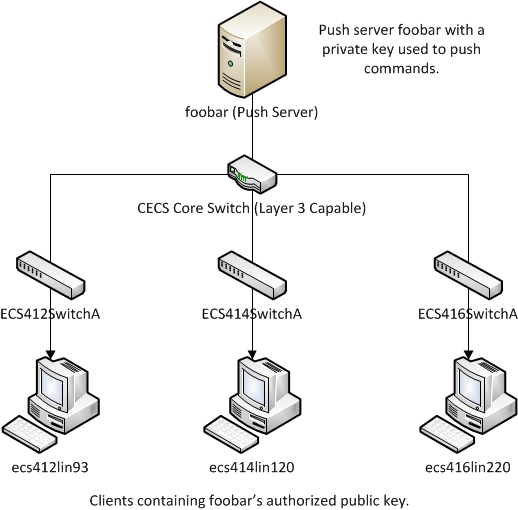
\includegraphics{../figures/sshpush.png}}
  \end{center}
  \caption{SSH Remote Command Push}
  \label{fig:sshpush}
\end{figure}

Because a password prompt never occurs, SSH can be used to run a command immediately after authentication.  With the use of semicolons and other special shell characters, multiple commands can be run.  Hypothetically, a command to download a script from a webserver can be followed by the command to run that script.  However, each system touched must have their public key accepted by the push server at least once to prevent prompts from occurring during automation.  For clones, it is useful to have all the clones use the same key.  And for subsequent clones, the previous key may be used to prevent SSH from failing due to a key identification mismatch.  This should not be done in highly secure environments though, as it circumvents protection against man in the middle attacks.  

\subsection{Push Script}
Thus, a relatively short script can be written to send commands to all participating servers.  In its simplest form, all this script does is loop through a list of hosts and execute the SSH command on each host.  In some shells, the loop may malfunction if SSH is not run in batch mode to prevent stdin, so care must be taken to remember that argument if using such a Unix shell.  

A more advanced script would fork each SSH command to the background to run commands on hosts in parallel.  This has the potential to overload the push server,\footnote{The push server is most likely to be a fairly old machine} so adding a delay after so many forked commands would help if the CPU is being taxed too much.  A fair amount of CPU cycles are used to negotiate the key exchange and encrypt the traffic.  The other issues that may occur are hosts that hang the SSH session.  This will cause the SSH command process to hang until killed.  Sometimes it can only be killed with signal 9.  If hosts do not seem to be doing this often, it may be fine to overlook and fix them manually after the script is run\footnote{We log the malfunctioning systems and investigate them later.}.  To remedy failed SSH sessions, at the end of the script, we force the script to sleep for a reasonable amount of time then kill all SSH sessions with the ``killall" command.  


\section{Unclogging}\label{sec:unclogging}
\subsection{Background}
Sometimes restricting privileges on lab machines is not enough to prevent students from clogging the machines.  If not locked down sufficiently, students can potentially cause headaches to system administrators.  Often, the students are not even malicious.  They could simply be doing assignments that have the potential to overload the lab machines.

For example, in an operating systems course, students must learn how to properly create, fork, kill, and end processes.  As with any programming, practice is needed to properly learn a new programming technique and many mistakes will be made along the way with each program run.  With operating systems concepts, many leftovers will remain after each program run.  Forking of processes will leave behind orphaned children if the program does not exit cleanly.  In addition, if a student's loop runs away, the potential for overloading the system with forked processes exists.  
\subsection{Limiting}
To prevent this, steps need to be taken to limit what a student can do.  For example, a student can run through a finite set of process IDs (PIDs) very quickly with a loop.  If the system does not have a limit for a single user to have, the user can make the system run out of PIDs.  By default, some Linux distributions set the kernel limit for a single user to 1024.  However, on other distributions and other types of Unix, this limit is not necessarily in place or is too high.  Thus, it is important to check this and set it accordingly.  It may be a good idea to drop the process count to below a hundred if the student does not require a window manager (which could also be useful for forcing students to learn good command line habits).  

In addition to PIDs, students can still clog the machine by using too much CPU, memory, or disk space.  CPU and memory usage can both be limited by editing kernel parameters by user.\footnote{On most Unix systems, CPU and memory usage are unlimited by default.}  Disk space can be limited by setting a quota on home directories.  However, users may still be able to write to temp directories and fill those up, so it is also useful to mount those directories from separate partitions of limited size.  Temp directories may still be important for operating system performance, so a cronjob to delete excess temp files may be necessary.  In the case of CECS labs, each machine can be cloned again within 10-15 minutes.  It may be simpler from an administration perspective to just let the students use the full resources of lab machines (minus administrative privileges) for programming.  
\subsection{Simplest Solution}
For many of these issues, the answer is simply to schedule a reboot every night.  This will clear all orphaned processes, interrupt any processes that could be using resources, and reset the environment.  This is very simple to do by making an entry in root's crontab.  The reboots should take place in the middle of the night during less used hours to prevent loss of work.  

This may create a few issues on some Linux distributions though.  On Ubuntu, the file system can get somewhat dirty after a few weeks and on reboot will mount the file system read-only if it detects errors.  To prevent this, we set it to do an FSCK (File System Check) if errors exist.  Delayed login mode is required for this though, but since students are prevented from manually rebooting the machines, this will not affect much.  It also helps that the reboots take place at night.  Lastly, the setup should not require and administrator to interact if problems are found.  We have set FSCK to fix errors automatically without asking for confirmation.  Instructions on how to do this can be found in \ref{install master appendix}.

Verbose mode is also very helpful for troubleshooting machines quickly especially while classes are in session.  A splash screen is nice when trying to hide confusing output from non-technical users, but in a room full of computer science students this really is not necessary.  

\section{Local Repository}\label{sec:local_repository}
\subsection{Background}
One of the future changes we could make is implementing a local software repository for our given Linux distribution.  A repository contains software packages and updates supported for a given distribution.  Whenever we build a master image or update it, it must go out to a distribution repository for what we need.  This can generate a huge amount of bandwidth for large package and update request lists.  In bandwidth limited environments, it would be a good idea to create a local repository on a server that workstations and servers can pull updates from instead of going out to the Internet.  This server would service these requests.  The reason we could potentially need it is because our workstations are not being updated during the semester.  For that, all 90 workstations would have to download the same set of updates.  This would cause unneeded and excessive bandwidth requests against the campus routers.  
\subsection{Possible Setups}
There are two types of repository servers that we can use.  A repository mirror downloads all packages and updates from a remote repository and stores them locally.  It updates itself periodically to be current.  It does require a significant bandwidth hit initially.  The currently mirror for Ubuntu requires about 30 GB.  This means we need that much hard disk space plus some extra in case it gets larger.  Disk space is not so much a problem as bandwidth though.  If the appropriate approvals for the initial bandwidth can be acquired, it will prevent the need for more bandwidth later.  There will still be a need for some bandwidth during updates, but it will be minimal.  
The other method is a repository cache.  Rather than mirroring an entire repository, this server acts as a middleman for repository requests.  Clients make a request to it for packages and updates.  It goes out to the remote repository and downloads it.  It then allows the client to download the package from it.  It does not remove the package though.  Instead, it caches it locally in case other clients need the same package.  Thus, if all 90 workstations need the same package, it is only downloaded once to the repository cache server who makes it available on the local network.  
We do not have a set of instructions for building it as we have not had the need to do so yet.  However, it does require that an apache webserver be set up because client machines download via the standard web protocol.  This may seem insecure, but the packages are one-way hashed and the matching hashes are downloaded initially via a secure connection and compared.  This also helps in the event of data corruption.  The repository mirror or cache is then shared via the apache web directory.  All clients can then be pointed to the webserver as their target repository.  In the case of mirroring, the last step is to set up periodic synchronization so that the local repository remains current.  We assume this is done automatically but a crontab entry can be created if necessary.
\subsection{Why Not Needed}
We do not use a local repository as of this writing.  For security reasons, our labs are relatively isolated from the rest of the world.  We therefore do not need immediate automatic updates.  This could become an issue if we choose a more targeted distribution, but we have not seen a security incident in our Linux labs as of yet (we are far more worried about our Windows environment).  The other reason we hesitate to implement it is because some software updates can break a course curriculum software.  For example, if our major development IDE Eclipse were to get an update mid-semester that changes its interface or breaks it, we would have confusion from the students and anger from the faculty.  Even security updates could potentially cause issues.  The reason we would consider it is in case a critical package is needed mid-semester that no one told us about.  Rather than clone the entire lab again, we would just need to run the package installation tool on the required workstations via an ssh push.  However, so far the need for it is mitigated by the fact that we build to a since master image and clone. This has been sufficient so far, but it would be nice to be able to update mid-semester if needed without taking down all of the workstations to perform the cloning. 


\section{Specialty Labs} \label{sec:specialty_labs}
\subsection{Overview}
General labs are not always sufficient for all applications.  Sometimes, specialty labs are necessary to do functions that general labs cannot do.  These labs will often have special requirements, such as unique equipment, a different network configuration, a different accounting system, and often a different room environment.  The labs we have covered consist of:  a system administration lab, a network administration lab, a computing cluster lab, a dedicated security lab, a terminal lab, a virtualized lab, and an individual projects lab. While these labs enhance our environment considerably, maintaining so many different configurations with such a limited staff becomes difficult. Thus, these labs are difficult to keep maintained permanently without faculty assistance.  
\subsystem{System Administration Lab}
The system administration lab is for teaching student system administrators (sysadmins).  Because they are given administrative privileges on their machines, they have a huge risk of causing damage or installing something malicious.  For that reason, this lab is isolated from outside networks and the Internet.  Students still need to do work remotely, and certain things must be brought into the lab, so a gateway server is set up with two network interfaces.  This server is open to the outside via one interface, but does not route traffic between the two.  This way, a student can remotely access the gateway, then from the gateway access the rest of the lab.  
\paragraph
Because of this isolation, the lab needs a Linux distribution that can be installed with all tools locally.  Certain distributions, such as Ubuntu, only offer a CD with the core installation and make administrators download what they need on top of it.  Since that is not an option in an isolated lab, a distribution that is fully offered on a CD or DVD set is needed.  In the CECS sysadmin lab, we use Slackware.  This is also arguably the best Linux distribution to teach system administration with because it makes administrators do everything manually.  From an efficiency standpoint, this is not ideal.  However, by making students do everything from scratch, it allows them to troubleshoot problems and truly understand what is going on.  
\paragraph
The sysadmin lab also needs more than 1 subnet in the lab.  For this, we use a second server to act as a 3 way router.  This division is necessary to separate the servers in the lab from the lab workstations, as well as to split the workstations up.  Since students have administrative privileges, they can potentially configure network settings wrong.  For example, if a student doing a system install assignment mistakenly gives their machine the address of the default gateway, they will cause the rest of the lab to send traffic to both them and the gateway.  By dividing the subnets up, they will only take down their subnet rather than the entire lab.  And they will not affect the servers.  It is still annoying to trace who actually did it but it is manageable.  It will also give the students practice with subnet calculations since they will have to work with small subnets under 8 bits.
\paragraph
As with the main labs, the sysadmin lab will need its own set of accounts, its own core servers, its own master image, and be cloned separately.  It needs accounts because the lab can not talk to the core servers for the rest of the labs.  In addition it will need a server to PXE boot from for clones (ideally, it would be the server that functions as a router in the lab).  Lastly, it would need its own master image.  The image would be simple, however, because one assignment in the labs would be rebuilding the image from scratch on individual machines.  It cannot be too complex, just enough to show some basic optimization and software installation choices that a good sysadmin should know.  
\subsection{Network Lab}
The network administration lab is very similar to the sysadmin lab except for a handful of other things.  This lab's purpose is to teach network fundamentals to students as well as troubleshooting and administration skills.  For research purposes, this lab would also be used to demonstrate applications of network theory.  
\paragraph
Since it will be dealing with network devices, the machines would benefit from having wireless cards to connect to wireless nodes.  It would be ideal if this lab were in a location where it would not interfere too heavily with other wireless infrastructures.  Many years ago, it was also useful for these workstations to support other network protocols.  However, since TCP/IP has become the standard across the board, this is no longer an issue.  
\paragraph
If this lab is teaching students home networking, they would benefit from the lab using the most common subnets:  192.168, 172.16, or 10.  In addition, this lab could not remain completely isolated since home networks expect to be able to reach the Internet.  Thus, a 2 way firewall can be used to restrict all inbound traffic behind a NAT (Network Address Translation) border.  It will also restrict outbound traffic to only the most common ports (web, ftp, ssh, etc.).  It should also be blocked from accessing other on-site resources and thus only have an avenue to the public Internet.  This will prevent the majority of issues with student network administrators.   
\subsection{Computing Cluster Lab}
A computing cluster is a set of machines working together to perform a complex computation.  This is a fundamental function for distributed computing.  They usually consist of a head node, which acts as the controller, and child nodes, which work together to perform calculations and communicate the results to the head node.  A lab of these machines requires special considerations.  
\paragraph
Often it is not a lab per se, but a server room full of racks.  This is not absolution necessary but it helps in situations where things can be automated.  In some clusters, there is no automation for the cluster software so each machine must be touched directly to add them to the cluster.  This is not very desirable, but it is common with software made by Adobe.  In this case, all the nodes would be workstations with monitors, keyboards, and mice.  This also makes it simpler to add hardware since you only need to set the hardware on a table and connect it rather than rack mount it.  
\paragraph
It is important that this lab has adequate cooling to support the heat these nodes will generate.  This is probably the most important aspect of the lab.  The room will hugely benefit from having a backup power supply (a generator or UPS) and a backup air conditioning system.  If the cluster is not well funded though, these things may not be necessary.  This would mean the cluster would be periodically shut down and hence would not be suitable for production work.  
\paragraph
The lab machines should have a very barebones operating system installation and only have the software used to run the cluster installed.  Anti-virus and other utility software that could use precious CPU cycles should not be installed.  As such, this lab would also benefit from being isolated from the outside world and have a gateway device people remotely login to.  It is a relatively insecure lab in that respect.  Access to this lab should be restricted only to the people using it for its designed purpose and it should not for any reason be used for general purpose computing (such as web browsing, email, etc.).  If it needs to go outside to download and upload finished computations, only the head node should be allowed to do it.  
\paragraph
Lastly, this lab needs a powerful network infrastructure.  Since these machines are working heavily with each other, the network becomes very chatty.  It should be using a switch (not a hub) with a high throughput.  A nice gigabit switch without QOS (quality of service) would work nicely.  Since this lab is relatively isolated, there is no point in giving them public IP addresses either, so they should be fine with a private 192.168 subnet.  
\paragraph
Given all the above, a dedicated cluster lab would be very costly both in funds available and in room/rack space.  Although CECS has a dedicated cluster occasionally, when we do not we compromise by allowing cluster software to run on our main Linux lab workstations.  Thus, one of our labs of 30 machines can be turned into a makeshift cluster so long as the cluster software does not require administrative rights.  
\subsection{Terminal Lab}
A terminal lab does not consist of workstations but of terminals.  Terminals (sometimes called dumb terminals) do not perform any work on their own.   Rather, they exist just to allow users to communicate with servers they are tied to.  Users do not do any work in terminal labs but instead connect to servers to do work there.  Terminals have not seen much use in recent years.  They were much more common when computers were much larger and could only fit in dedicated machine rooms.\footnote{Mainframes were a perfect example of this}  However, users can still use lab workstations to do work on servers with network clients.  For example, a lab could consist of very weak Linux workstations that only provide students with an ssh client.  They were ssh to a server in another room and use that server's compiler to develop code.  Alternative, they could use a remote desktop client to communicate with Windows Terminal Servers to use Windows-only applications.  These labs are relatively easy to manage because they have very simple purposes.  Actually setting up the servers they connect to represents the bulk of the workload for administrators.  
\subsection{Dedicated Security Lab}
A dedicated security lab is for teaching students about system and network security as well as potentially prepare them to become penetration testers (pen testers).  This lab could also be used to test and analyze malware.  As such, there is no reason this lab should not be completely isolated.  Even a gateway server to access it remotely is a risk because the gateway server could become compromised.  If the lab absolutely has to be accessed remotely, it should be through a remote KVM console that only allow a user to see screen output and pass keyboard strokes (no network traffic allowed).  Other aspects of this lab are beyond the scope of this thesis.  
\subsection{Virtual Machine Lab}
This lab does not take up space in room.  Rather, very spacious servers host virtual machines (VMs) that users access only remotely.  These servers must have a lot of CPU, Memory, and Hard Disk space to support operating systems running on top of them.  The advantage to this environment is very easy deployment of VMs from clone images.  All work can (and should) be done remotely and with automation.  In addition, because they are virtualized, they can be torn down and replaced quickly if a problem emerges.  The disadvantage is these VMs can not quite reach the performance of separate physical hosts.  In addition, if the VM host is not set up to properly schedule resources, one VM can potentially take up most of the resources available and slow down all other VMs on the host.  
\subsection{Individual Projects Lab}
Lastly, it is useful to have a lab solely dedicated to individual projects.  In CECS, we have a dedicated senior projects and graduate student lab that students can use to work in.  This lab may be the most difficult to manage because there are so many different project students do in this lab.  They may or may not even need workstations or network access but instead just need a space and tools to work on hardware.  Determination on how to manage this lab should be on a project by project basis.  Each student should have some sort of project plan or charter and hold discussions with lab managers on what exactly they plan to do.  Communication with the users is more important than anything else in this sort of lab environment as each project team may have special needs.  

\section{Crossplatform Considerations} \label{sec:crossplatform}
\subsection{Background}
Up until now, only Linux based labs have been described.  However, to be competitive in today's market, many platforms need to be considered.  In CECS, we have a combination of Windows, Mac OSX, and various distributions of Linux.   Getting all of them to play nicely with each can often be an aggravating (sometimes maddening) process.  In addition, the choice of platforms is often dictated by people other than the System Administrators. 
\subsection{Centralized Accounting}
The most important thing to consider in a mixed platform environment is the user accounting system.  This is the system that manages login user IDs, user attributes, and passwords.  User attributes may consist of a user's full name, student/employee name, contact email, etc.  Some other useful attributes could be a list of courses that student takes or what his major is.  

At the very least, the system needs to manage user IDs and passwords centrally.  If this is not done, each platform must have its own central authentication system set up and each user must remember separate sets of user IDs and passwords (though the users may set them all the same).  This will also make shared resources among the different platforms difficult to use securely.  File servers in particular need a central authentication mechanism to know which files are owned by whom.  

There are two choices for central authentication that we have looked into.  The first is Network Information Services (NIS) with its set of yp commands.  This was created by Sun Microsystems as a method to exchange network and directory information between Unix systems.  The advantage to it is that every flavor of Unix supports it and will share passwd file information easily.  The disadvantage to it is that is shares information in clear text form.  This becomes a problem because password hash values can be sniffed if the network is breeched.  The other disadvantage is it will not natively support Microsoft Windows systems.  

The second choice is Microsoft Active Directory.  This is Microsoft's method for sharing information across Windows systems.  It can be difficult to configure but it is the ideal (and only) choice in a pure Windows environment.  The disadvantage is that Unix systems can not usually use it.  There have been many attempts at achieving compatibility and we are currently looking into another one, but no smooth tool has yet been made to fully support all of Microsoft's features.  

What we have done in CECS labs is have NIS manage authentication and created our own system to transfer credentials to a Windows Active Directory domain controller (sometimes called a PDC).  Unix clients can bind natively to an NIS namemaster while Windows clients must bind through Active Directory (AD).  Thus, we need two types of authentication: NIS and AD.  Our solution to this is called the search program.  We have a special user account called ``search" with the password ``account" that is the only method students can use to create their user accounts.  This program stores the usernames and passwords that students create in a clear text file temporarily.  This file is allowed to be read by another account called ntamaker (NT Account Maker).  This account is used from the PDC to access this clear text file.  Every 15 minutes, the PDC remotely copies the accounts in this file and adds them to its Active Directory accounts.  This is possible because it has access to clear text passwords for a brief period.  After it creates the accounts, it overwrites the file and erases the password information.

With the common accounts in place, we can then implement centralized file systems.  Since user IDs between different platforms are not usually the same, we are forced to go strictly by username.  This requires that all usernames are unique across all of our platforms.  It has not been an issue for CECS but it could potentially be for other environments.  With the usernames in place, the file servers can use them to distinguish who owns which files.  Thus, when users authenticate to either the NIS namemaster or the PDC, they are allowed to access files that they own.  The other problem that arises is incompatibility between Windows and Unix NFS.  Windows can only mount Samba shares.  This is fixed by running a Samba server on the printservers which is further described in detail in Chapter~\ref{ch:lab_infrastructure}, Section~\ref{sec:printservers}.  

\subsection{Software}
Even though a platform may not always work nicely with another platform, a lot of software has been ported to work across different platforms.  This is nice because certain labs can then be scheduled for use with multiple courses in a curriculum.  For example, Adobe's Web Development Suite has been ported to both Windows and Macintosh platforms.  So either lab can be scheduled for Web Development courses.  Eclipse and other Java based applications work on all platforms that a Java interpreter has been ported to.  This allows some flexibility in lab schedules so that courses that need platform specific software can get it more easily.  In addition, a lab may be able to remotely access servers of another platform.  For example, the Linux labs can be scheduled to use a Windows specific piece of software because students can use the ``rdesktop" command to remotely use a Windows Terminal Server.  

\subsection{Issues}
Issues with multiple platforms are many and varied.  It would be impossible to describe all of the issues we have faced, so I will give some of the more common examples.  

The biggest issue by far occurs when one platform updates and breaks compatibility with another platform.  For example, often during Apple OS X updates, either Samba, NFS, or NIS stops working as it did in previous versions.  Apple sometimes releases fixes after complaints, but we have had to do our own workarounds usually.  For example, when Samba broke, we could no longer bind the Macs to a Windows PDC.  We instead had to bind them to our Unix NIS namemaster.  However, the Macs could not support user home directories being NFS mounted.  After only a few minutes, the workstations would hang with no warning and have to be hard rebooted.  In addition, the error codes had no documentation available to help troubleshoot.  As a workaround, we mounted the directories to an alternate location and created a symbolic link to them.  However, in Apple's next release, even this workaround did not help because NIS was broken.  We ended up having to downgrade the workstations until Apple could release a patch six months later.

Another issue is the occasional failure to do Samba mounts.  This happens because Samba has an operation called an oplock for which NFS does not have an equivalent capability.  We have been able to mostly fix this issue by having the Samba server on the printservers fake oplocks.  We still occasionally have issues but they are minor.  

We also had trouble finding a client on Windows that could communicate via ssh or telnet easily.  When we upgraded to Windows 7, the Hyperterm program was removed.  We eventually found the Putty program that could use ssh and give shell access to Linux servers, but it did not have some of the features that we were used to in Hyperterm.  This invalidated the instruction sets we gave to faculty and caused confusion while we updated.  

\chapter{Conclusion} \label{ch:conclusion}
\section{Summary} \label{sec:summary}
In conclusion, managing the CECS labs is a difficult task made easier by using efficient management.  We have problems to resolve on all fronts from tedious deployments to constant updates.  This is all made easier through automation and careful crafting of our infrastructure.  

%For documentation, we use a shared user account and store instructions there.  We maintain a support website and shared technical support email.  Our infrastructure consists of fileservers and printservers.  Our install process involves creating a master lab image and cloning it to many workstations over the network.  Maintenance during the semester is done via Secure Shell pushes and periodic automated cleaning.  Lastly, we maintain a mixed environment with many different platforms across regular labs and specialty labs.  Maintaining all of this can be challenging, but we make it easier through automation. 

As far as common university problems, we have handled most of them.  Our permissions limit students and faculty sufficiently while still allowing them to do work in a technical field.  We handled the paper accounting problem by creating the paperd program and connecting printers to print servers.  All of our main labs are uniformly based on clones of a master image which saves considerable time and effort customizing each one.  Although we have many special labs, the same master image and clone techniques are used in each one to facilitate efficient management and we have had faculty to support to assist us.  Student data is highly available as we have 2 different backup servers back up every night.  Down time is very rare because our file servers are well maintained and very reliable.  And although crossplatform interoperability has always had a significant time cost, we have so far managed to find solutions by combining our experience.

It is important to note that our solutions are not the only solutions.  Other universities may be run very differently.  Some universities build their infrastructure with a Microsoft Windows based core instead of Linux.  Others may have chosen to standardize completely on one platform to avoid the various issues we have faced.  The technical details given in this paper's appendix section have probably been written very differently at other universities.  However, the fundamental concept of automation where possible in addition to building a solid core is of great importance not just in universities but in other IT environments. 



%\appendix
%\include{phonyAppendixA} %-Use this to make a thesis office approved TOC, LOF, and LOT
%\include{phonyAppendixB} %-Use this to make a thesis office approved TOC, LOF, and LOT
% \include{detailedDescriptionOfTheCircuit}
% \include{circuitConstruction}

%\bibliographystyle{utphys}  % With journal title
% \bibliographystyle{h-physrev} % No journal title appears
% \bibliography{papers}
%\include{bibliography}
\end{document}
%%                                                            %%
%%------------- End of Document ------------------------------%%
